%------------------------------------------------------------
\title[01 - 函数 I]
{01 - 函数 I}

\subtitle{C++ 程序设计进阶}

\author[Beiyu Li]
{Beiyu Li\\
\texttt{<sysulby@gmail.com>}}

% \institute[SOJ]
% {Sicily Online Judge}

\date[\today]
{\number\year 年 \number\month 月 \number\day 日}
%------------------------------------------------------------


\begin{document}

\author[sysulby]
{SOJ 信息学竞赛教练组}

\begin{frame}
    \titlepage
\end{frame}
\setcounter{framenumber}{0} % 标题页不编号

\section{引入函数}

%------------------------------------------------------------
\begin{frame}[fragile]
    \frametitle{讨论}

    \begin{block}{}
        \vspace{.5cm}
        \begin{center}
            {\Large 什么是函数?}
        \end{center}
        \vspace{.5cm}
    \end{block}
\end{frame}
%------------------------------------------------------------

%------------------------------------------------------------
\begin{frame}[fragile]
    \frametitle{函数}

    \begin{itemize}
        \item<1-> 数学中的函数:一个变量 $y$ 随另一个变量 $x$ 的变化而变化
        \begin{itemize}
            \item<1-> 例如:$y = 2x + 1$ 中 $x$ 为自变量,$y$ 为因变量
        \end{itemize}
        \item<2-> 编程中的函数:一系列代码,用于\textbf{实现某个特定的功能}
        \begin{itemize}
            \item<2-> 接收\textbf{给定的自变量},通过该函数处理,得到特定的\textbf{结果(因变量或效果)}
        \end{itemize}
    \end{itemize}
\end{frame}
%------------------------------------------------------------

\section{函数的定义与调用}

%------------------------------------------------------------
\begin{frame}[fragile]
    \frametitle{函数的定义}

    \begin{itemize}
        \item<1-> 函数的定义形式如下:
        \uncover<1->{\lstinputlisting[basicstyle=\ttfamily\scriptsize,language=C++,name=functionStructure1]{ch13/functionStructure1.cc}}
        \item<2-> 函数的定义需要写在 \textbf{\lstinline|main| 函数外面}
        \item<3-> 确定函数的\textbf{功能},把功能的实现写在函数体中
        \uncover<4>{\lstinputlisting[basicstyle=\ttfamily\scriptsize,language=C++,name=print]{ch13/print.cc}}
    \end{itemize}
\end{frame}
%------------------------------------------------------------

%------------------------------------------------------------
\begin{frame}[fragile]
    \frametitle{例 1.1:输出一行 hello world}
        \begin{exampleblock}{编程题}

            \begin{itemize}
                \item 请定义一个 \lstinline|print| 函数,功能:输出一行 \lstinline|hello world|。\\
                    在主函数调用该函数,实现输出。

                \item 样例输入

                    无

                \item 样例输出

                    \lstinline|hello world|

            \end{itemize}

        \end{exampleblock}
\end{frame}
%------------------------------------------------------------

%------------------------------------------------------------
\begin{frame}[fragile]
    \frametitle{函数的实现}

    \begin{itemize}[<+->]
        \item 函数名的命名规则与变量名的命名规则相同
        \item 函数名后面的小括号不能省略
        \item 函数体是函数功能的具体实现:输出一行 \lstinline|hello world|

        \lstinputlisting[basicstyle=\ttfamily\scriptsize,language=C++,name=print]{ch13/print.cc}
    \end{itemize}
\end{frame}
%------------------------------------------------------------

%------------------------------------------------------------
\begin{frame}[fragile]
    \frametitle{函数的调用}

    \begin{itemize}[<+->]
        \item 定义函数后,需要用调用语句来执行函数
        \item 函数的调用语句为:\textbf{函数名()}
        \begin{itemize}
            \item 调用函数时不能省略小括号
        \end{itemize}

        \item 函数体中可以调用任何前面已经定义的函数
        \begin{itemize}
            \item \lstinline|print| 函数定义在 \lstinline|main| 函数之前,故可在 \lstinline|main| 函数中调用
            \item 特殊地,在程序启动时会自动调用 \lstinline|main| 函数
        \end{itemize}
    \end{itemize}
\end{frame}
%------------------------------------------------------------

%------------------------------------------------------------
\begin{frame}[fragile]
    \frametitle{例 1.1:输出一行 hello world}
    
    \lstinputlisting[basicstyle=\ttfamily\scriptsize,language=C++,name=printHelloWorld]{ch13/printHelloWorld.cc}
\end{frame}
%------------------------------------------------------------

%------------------------------------------------------------
\begin{frame}[fragile]
    \frametitle{讨论}

    \begin{block}{}
        \vspace{.5cm}
        \begin{center}
            {\Large 如何让函数输出 n 行 hello world 呢?}
        \end{center}
        \vspace{.5cm}
    \end{block}
\end{frame}
%------------------------------------------------------------

%------------------------------------------------------------
\begin{frame}[fragile]
    \frametitle{函数的多次调用}
    
    \lstinputlisting[basicstyle=\ttfamily\scriptsize,language=C++,name=n_calls]{ch13/n_calls.cc}
    \begin{itemize}
        \item<2-> 一次函数调用能否输出多行?
    \end{itemize}
\end{frame}
%------------------------------------------------------------

\section{函数的参数}

%------------------------------------------------------------
\begin{frame}[fragile]
    \frametitle{函数的进阶写法}

    \begin{itemize}[<+->]
        \item 函数的定义形式可以调整为:
        \lstinputlisting[basicstyle=\ttfamily\scriptsize,language=C++,name=functionStructure2]{ch13/functionStructure2.cc}
        \item \textbf{参数列表} 相当于 “给定的自变量”,接收实现函数功能所需的数据
        \item 之前写的函数都是 参数列表为空 的情况
    \end{itemize}
\end{frame}
%------------------------------------------------------------

%------------------------------------------------------------
\begin{frame}[fragile]
    \frametitle{参数列表}

    \begin{itemize}
        \item 参数列表可以为空
        \item 参数列表可以不为空
        \begin{itemize}
            \item 要说明每个参数的\textbf{参数类型、参数名}
            \item 参数类型可以是 \lstinline|int, long long, double, char, ...| 
        \end{itemize}
    \end{itemize}
\end{frame}
%------------------------------------------------------------

%------------------------------------------------------------
\begin{frame}[fragile]
    \frametitle{例 1.2:输出 5 行 hello world}
        \begin{exampleblock}{编程题}

            \begin{itemize}
                \item 请定义一个 \lstinline|print| 函数,功能:输出 $n$ 行 \lstinline|hello world|。\\
                    在主函数调用该函数,实现输出 $5$ 行 \lstinline|hello world|。

                \item 样例输入

                    无

                \item 样例输出

                    \lstinline|hello world|\\
                    \lstinline|hello world|\\
                    \lstinline|hello world|\\
                    \lstinline|hello world|\\
                    \lstinline|hello world|

            \end{itemize}

        \end{exampleblock}
\end{frame}
%------------------------------------------------------------

%------------------------------------------------------------
\begin{frame}[fragile]
    \frametitle{有参数的函数实现}

    \begin{itemize}[<+->]
        \item 函数体是函数功能的具体实现:输出 $n$ 行 \lstinline|hello world|
        \item 其中,$n$ 是实现函数功能所需接收的数据,故为函数的参数,其类型为整数

        \lstinputlisting[basicstyle=\ttfamily\scriptsize,language=C++,name=printNHello]{ch13/printNHello.cc}
    \end{itemize}
\end{frame}
%------------------------------------------------------------

%------------------------------------------------------------
\begin{frame}[fragile]
    \frametitle{有参数函数的调用}

    \begin{itemize}[<+->]
        \item 有参数函数的调用语句为:\textbf{函数名(参数)}
        \item 调用有参数的函数时,参数应为具体的数值或变量
        \begin{itemize}
            \item \lstinline|print(5);| 表示调用函数,输出 $5$ 行 \lstinline|hello world|
            \item \lstinline|int x = 10;|\\
                  \lstinline|print(x);| 表示调用函数,输出 $x$($10$) 行 \lstinline|hello world|
        \end{itemize}
    \end{itemize}
\end{frame}
%------------------------------------------------------------

%------------------------------------------------------------
\begin{frame}[fragile]
    \frametitle{例 1.2:输出 5 行 hello world}
    
    \lstinputlisting[basicstyle=\ttfamily\scriptsize,language=C++,name=printNHelloWorld]{ch13/printNHelloWorld.cc}
\end{frame}
%------------------------------------------------------------

%------------------------------------------------------------
\begin{frame}[fragile]
    \frametitle{随堂练习}

    \begin{exampleblock}{找错题}

        \begin{enumerate}
                \only<1-2>{
                \item[1.] 阅读程序,找出代码中的错误
                    \lstinputlisting[basicstyle=\ttfamily\scriptsize,language=C++,name=exercise1]{ch13/exercise1.cc}

                    \begin{tikzpicture}[remember picture,overlay]
                        \uncover<2>{\redbox{exercise1}{7}{1}{7}{8}  node[right,yshift=0.2cm]{\lstinline|该语句不会被执行|};}
                    \end{tikzpicture}
                }

                \only<3-4>{
                \item[2.] 阅读程序,找出代码中的错误
                    \lstinputlisting[basicstyle=\ttfamily\scriptsize,language=C++,name=exercise2]{ch13/exercise2.cc}
                    
                    \begin{tikzpicture}[remember picture,overlay]
                        \uncover<4>{\redbox{exercise2}{8}{3}{8}{8} node[right,yshift=0.2cm]{\lstinline|不能省略小括号|};}
                    \end{tikzpicture}

                }

                \only<5-6>{
                \item[3.] 阅读程序,找出代码中的错误
                    \lstinputlisting[basicstyle=\ttfamily\scriptsize,language=C++,name=exercise3]{ch13/exercise3.cc}
                    
                    \begin{tikzpicture}[remember picture,overlay]
                        \uncover<6>{\redbox{exercise3}{10}{3}{10}{10} node[right,yshift=0.2cm]{\lstinline|需要传参|};}
                    \end{tikzpicture}
                }
        \end{enumerate}

    \end{exampleblock}
\end{frame}
%------------------------------------------------------------

%------------------------------------------------------------
\begin{frame}[fragile]
    \frametitle{讨论}

    \begin{block}{}
        \vspace{.5cm}
        \begin{center}
            {\Large 如果函数需要返回某个结果,该如何实现呢?}
        \end{center}
        \vspace{.5cm}
    \end{block}
\end{frame}
%------------------------------------------------------------

\section{函数的返回值}

%------------------------------------------------------------
\begin{frame}[fragile]
    \frametitle{函数的进阶写法}

    \begin{itemize}[<+->]
        \item 函数的定义形式可以调整为:
        \lstinputlisting[basicstyle=\ttfamily\scriptsize,language=C++,name=functionStructure]{ch13/functionStructure.cc}
        \item 没有返回值时,其返回值类型为 \lstinline|void|,这样的函数称为 “无返回值的函数”
        \item 返回值类型为 其他数据类型时,这样的函数称为 “有返回值的函数”
        \item 之前写的函数都是 无返回值的函数
    \end{itemize}
\end{frame}
%------------------------------------------------------------

%------------------------------------------------------------
\begin{frame}[fragile]
    \frametitle{返回值}

    \begin{itemize}
        \item 返回值 相当于 函数执行后得到的 “\textbf{因变量(结果)}”
        \item 返回值可以为空
        \item 返回值可以不为空
        \begin{itemize}
            \item 根据结果的类型确定返回值类型
            \item 返回值类型可以是 \lstinline|int, long long, double, char, ...| 
            \item 返回值由 \textbf{\lstinline|return|} 语句返回
        \end{itemize}
    \end{itemize}
\end{frame}
%------------------------------------------------------------

%------------------------------------------------------------
\begin{frame}[fragile]
    \frametitle{例 1.3:输出从 1 到 n 的整数之和}
        \begin{exampleblock}{编程题}

            \begin{itemize}
                \item 请定义一个 \lstinline|getSum| 函数,功能:计算 $1 \sim n$ 的和。\\
                    输入一个正整数 $n$($1 \le n \le 1000$),输出 $1 \sim n$ 的和。

                \item 样例输入

                    \lstinline|100|

                \item 样例输出

                    \lstinline|5050|

            \end{itemize}

        \end{exampleblock}
\end{frame}
%------------------------------------------------------------

%------------------------------------------------------------
\begin{frame}[fragile]
    \frametitle{有返回值函数的实现}

    \begin{itemize}[<+->]
        \item 函数体是函数功能的具体实现:计算 $1 \sim n$ 的和
        \item 其中,$n$ 是实现函数功能所需接收的数据,故为函数的参数,其类型为整数
        \item 其中,“和” 是函数执行后需要得到的结果,故为函数的返回值,其类型为整数,使用 \lstinline|return| 语句返回

        \lstinputlisting[basicstyle=\ttfamily\scriptsize,language=C++,name=getSum]{ch13/getSum.cc}
    \end{itemize}
\end{frame}
%------------------------------------------------------------

%------------------------------------------------------------
\begin{frame}[fragile]
    \frametitle{有返回值函数的调用}

    \begin{itemize}[<+->]
        \item 有返回值函数的调用语句与无返回值函数的调用语句一致
        \item 有返回值函数调用时,可将其视作具体的数值进行运算或输出
        \begin{itemize}
            \item \lstinline|int sum = getSum(5);| 表示调用函数,计算 $1 \sim 5$ 的和,并将和存入 \lstinline|sum| 中
            \item \lstinline|cout << getSum(5) << endl;| 表示调用函数,计算 $1 \sim 5$ 的和,并将和输出
        \end{itemize}
    \end{itemize}
\end{frame}
%------------------------------------------------------------

%------------------------------------------------------------
\begin{frame}[fragile]
    \frametitle{例 1.3:输出从 1 到 n 的整数之和}
    
    \lstinputlisting[basicstyle=\ttfamily\scriptsize,language=C++,name=print_1_n_sum]{ch13/print_1_n_sum.cc}
\end{frame}
%------------------------------------------------------------

%------------------------------------------------------------
\begin{frame}[fragile]
    \frametitle{随堂练习}

    \begin{exampleblock}{找错题}

        \begin{enumerate}
                \only<1-2>{
                \item[1.] 阅读程序,找出代码中的错误
                    \lstinputlisting[basicstyle=\ttfamily\scriptsize,language=C++,name=exercise4]{ch13/exercise4.cc}                

                    \begin{tikzpicture}[remember picture,overlay]
                        \uncover<2>{\redbox{exercise4}{12}{3}{12}{12}  node[right,yshift=0.2cm]{\lstinline|运行结果无作用,程序无输出|};}
                    \end{tikzpicture}
                }

                \only<3-4>{
                \item[2.] 阅读程序,找出代码中的错误
                    \lstinputlisting[basicstyle=\ttfamily\scriptsize,language=C++,name=exercise5]{ch13/exercise5.cc}
                    
                    \begin{tikzpicture}[remember picture,overlay]
                        \uncover<4>{\redbox{exercise5}{8}{3}{8}{13};}
                        \uncover<4>{\redbox{exercise5}{4}{3}{4}{20};}
                        \uncover<4>{\redbox{exercise5}{3}{1}{3}{3}  node[above,xshift=2.8cm,yshift=0.2cm]{\lstinline|类型不正确,类型转换后数据溢出|};}
                    \end{tikzpicture}
                }
        \end{enumerate}

    \end{exampleblock}
\end{frame}
%------------------------------------------------------------

%------------------------------------------------------------
\begin{frame}[fragile]
    \frametitle{小结:函数的定义与调用}

    \begin{itemize}[<+->]
        \item 函数的完整框架为:

        \lstinputlisting[basicstyle=\ttfamily\scriptsize,language=C++,name=functionStructure]{ch13/functionStructure.cc}

        \item 函数是否有参数,取决于实现函数功能时是否需要接收数据
        \item 有参数的函数,调用时需要传入具体的数值
        \item 函数是否有返回值,取决于函数是否需要得到一个计算结果
        \item 有返回值的函数,调用时需要注意处理返回的结果,如进行运算或输出
    \end{itemize}
\end{frame}
%------------------------------------------------------------

\section{函数调用时的执行过程}

%------------------------------------------------------------
\begin{frame}[fragile]
    \frametitle{函数的调用}

    \begin{itemize}
        \item 函数体中可以调用任何前面已定义的函数
        \item 当执行到函数的调用语句时,程序将跳转到该函数中,执行其函数体的语句,直到执行完函数体或执行到 \lstinline|return| 语句。待函数执行完,程序会跳转回原调用处继续往下执行。
    \end{itemize}
\end{frame}
%------------------------------------------------------------

%------------------------------------------------------------
\begin{frame}[fragile]
    \frametitle{示例:无返回值函数的执行过程}

    \begin{columns}
        \column{.01\textwidth}

        \column{.63\textwidth}
        \lstinputlisting[basicstyle=\ttfamily\scriptsize,language=C++,name=void_function]{ch13/void_function.cc}
        \begin{tikzpicture}[remember picture,overlay]
            \uncover<2-5>{\redbox{void_function}{14}{3}{14}{14};}
            \uncover<3>{\redbox{void_function}{3}{1}{3}{18};}
            \uncover<3>{\draw[red, very thick, ->] ([shift={(2pt, .25em)}] pic cs:line-void_function-14-end) -- ++(12em, 0) |- ([shift={(2pt, .25em)}] pic cs:line-void_function-3-end);}
            \uncover<4>{\redbox{void_function}{4}{3}{4}{31};}
            \uncover<5>{\redbox{void_function}{5}{1}{5}{1};}
            \uncover<5>{\draw[red, very thick, ->] ([shift={(2pt, .25em)}] pic cs:line-void_function-5-end) -- ++(18em, 0) |- ([shift={(2pt, .25em)}] pic cs:line-void_function-14-end);}
            \uncover<6-9>{\redbox{void_function}{15}{3}{15}{15};}
            \uncover<7>{\redbox{void_function}{7}{1}{7}{23};}
            \uncover<7>{\draw[red, very thick, ->] ([shift={(2pt, .25em)}] pic cs:line-void_function-15-end) -- ++(12em, 0) |- ([shift={(2pt, .25em)}] pic cs:line-void_function-7-end);}
            \uncover<8>{\redbox{void_function}{8}{3}{10}{37};}
            \uncover<9>{\redbox{void_function}{11}{1}{11}{1};}
            \uncover<9>{\draw[red, very thick, ->] ([shift={(2pt, .25em)}] pic cs:line-void_function-11-end) -- ++(12em, 0) |- ([shift={(2pt, .25em)}] pic cs:line-void_function-15-end);}
            \uncover<10>{\redbox{void_function}{16}{3}{16}{11};}
        \end{tikzpicture}

        \column{.36\textwidth}
        \begin{itemize}                
                \item 执行过程\\
                    \only<3-4> {主函数执行暂停,等待 \lstinline|function1| 函数执行\\}
                    \only<5-6> {\lstinline|function1| 函数执行完毕,回到主函数继续执行\\}
                    \only<7-8> {主函数执行暂停,把 $3$ 赋值给 $n$,等待 \lstinline|function2| 函数执行\\}
                    \only<9> {\lstinline|function2| 函数执行完毕,回到主函数继续执行\\}
                    \only<10> {程序结束\\}
            
                \item 输出\\
                    \uncover<4->{\lstinline|function 1|\\}
                    \uncover<8->{\lstinline|function 2|\\}
                    \uncover<8->{\lstinline|function 2|\\}
                    \uncover<8->{\lstinline|function 2|\\}
                
        \end{itemize}
    \end{columns}
\end{frame}
%------------------------------------------------------------

%------------------------------------------------------------
\begin{frame}[fragile]
    \frametitle{示例:有返回值函数的执行过程}

    \begin{columns}
        \column{.01\textwidth}

        \column{.63\textwidth}
        \lstinputlisting[basicstyle=\ttfamily\scriptsize,language=C++,name=int_function]{ch13/int_function.cc}
        \begin{tikzpicture}[remember picture,overlay]
            \uncover<2>{\redbox{int_function}{12}{3}{12}{8};}
            \uncover<3>{\redbox{int_function}{13}{3}{13}{11};}
            \uncover<4-6>{\redbox{int_function}{14}{13}{14}{22};}
            \uncover<4>{\draw[red, very thick, ->] ([shift={(2pt, .25em)}] pic cs:line-int_function-14-end) -- ++(8em, 0) |- ([shift={(2pt, .25em)}] pic cs:line-int_function-3-end);}
            \uncover<4>{\redbox{int_function}{3}{1}{3}{19};}
            \uncover<5>{\redbox{int_function}{4}{3}{7}{32};}
            \uncover<6>{\redbox{int_function}{8}{3}{8}{13};}
            \uncover<6>{\draw[red, very thick, ->] ([shift={(2pt, .25em)}] pic cs:line-int_function-8-end) -- ++(8em, 0) |- ([shift={(2pt, .25em)}] pic cs:line-int_function-14-end);}
            \uncover<7>{\redbox{int_function}{14}{3}{14}{22};}
            \uncover<8>{\redbox{int_function}{15}{3}{15}{22};}
            \uncover<9>{\redbox{int_function}{16}{3}{16}{11};}
        \end{tikzpicture}

        \column{.36\textwidth}
        \begin{itemize}
                \item 输入\\
                \lstinline|3|
                
                \item 执行过程\\
                    \only<3> {输入 $x$ 的值,值为 $3$\\}
                    \only<4> {主函数执行暂停,把 $x$ 赋值给 $n$,等待 \lstinline|getSum| 函数执行\\}
                    \only<5> {计算得到 $sum = 6$\\}
                    \only<6> {返回值为 $6$,回到主函数继续执行\\}
                    \only<7> {把 $6$ 赋值给 $ans$\\}
                    \only<8> {输出 $ans$\\}
                    \only<9> {程序结束\\}

                \item 输出\\
                \uncover<8->{6}
        \end{itemize}
    \end{columns}
\end{frame}
%------------------------------------------------------------

%------------------------------------------------------------
\begin{frame}[fragile]
    \frametitle{形参与实参}

    \begin{itemize}
        \item 调用函数需要使用函数名,并把实际使用的参数放在括号中传递进去
        \item \textbf{形式参数}:函数定义时在括号里定义的变量,它只作为\textbf{指代}
        \item \textbf{实际参数}:调用函数时传给形参的\textbf{具体数值}
    \end{itemize}
\end{frame}
%------------------------------------------------------------

%------------------------------------------------------------
\begin{frame}[fragile]
    \frametitle{示例:有返回值函数的执行过程}

        \lstinputlisting[basicstyle=\ttfamily\scriptsize,language=C++,name=printNHelloWorld]{ch13/printNHelloWorld.cc}
        \begin{tikzpicture}[remember picture,overlay]
            \uncover<2>{\redbox{printNHelloWorld}{12}{3}{12}{11};}
            \uncover<2>{\redbox{printNHelloWorld}{5}{1}{5}{19};}
            \uncover<2>{\draw[red, very thick, ->] ([shift={(2pt, .25em)}] pic cs:line-printNHelloWorld-12-end) -- ++(12em, 0) |- ([shift={(6pt, .25em)}] pic cs:line-printNHelloWorld-5-end);}
            \uncover<3>{\redbox{printNHelloWorld}{12}{9}{12}{9} node[right,xshift=.2cm,yshift=-.2cm]{实际参数};}
            \uncover<3>{\redbox{printNHelloWorld}{5}{12}{5}{16} node[right,xshift=.2cm,yshift=.5cm]{形式参数};}
            \uncover<3>{\draw[red, very thick, ->] ([shift={(-2pt, .25em)}] pic cs:line-printNHelloWorld-12-end) -- ++(12em, 0) |- node[right,yshift=-1cm] {n = 5}([shift={(0pt, .25em)}] pic cs:line-printNHelloWorld-5-end);}
        \end{tikzpicture}

\end{frame}
%------------------------------------------------------------

%------------------------------------------------------------
\begin{frame}[fragile]
    \frametitle{参数列表}

    \begin{itemize}
        \item 函数的参数列表也可以有多个参数
        \item \textbf{每个参数}都要说明其\textbf{数据类型}和\textbf{参数名},不能省略
        \item \textbf{参数}之间使用\textbf{逗号}隔开
        \item 调用函数时,函数的\textbf{实际参数}需要和\textbf{形式参数}的\textbf{顺序一致}
    \end{itemize}
\end{frame}
%------------------------------------------------------------


%------------------------------------------------------------
\begin{frame}[fragile]
    \frametitle{例 1.4:求梯形的面积}

    \alt<2-3>{
        \lstinputlisting[basicstyle=\ttfamily\scriptsize,language=C++,name=ladder_shaped]{ch13/ladder_shaped.cc}
        \begin{tikzpicture}[remember picture,overlay]
            \uncover<3>{\redbox{ladder_shaped}{13}{17}{13}{39};}
            \uncover<3>{\redbox{ladder_shaped}{6}{1}{6}{52};}
            \uncover<3>{\draw[red, very thick, ->] ([shift={(2pt, .25em)}] pic cs:line-ladder_shaped-13-end) -- ++(9em, 0) |- node[right,yshift=-1cm,text width=1.2cm] {a = x b = y h = z}([shift={(4pt, .25em)}] pic cs:line-ladder_shaped-6-end);}
        \end{tikzpicture}
    }{
        \begin{exampleblock}{编程题}

            \begin{itemize}
                \item 已知梯形的面积公式为 $S = \frac{(a+b)h}{2}$,其中 $a, b, h$ 分别为上底、下底、高。\\
                    请定义一个 \lstinline|ladder_shaped| 函数,功能:用梯形的上底、下底和高,计算梯形的面积。\\
                    输入三个实数,表示梯形的上底、下底、高,输出梯形的面积,输出保留两位小数。

                \item 样例输入

                    \lstinline|1.5 2.5 3|

                \item 样例输出

                    \lstinline|6.00|

            \end{itemize}

        \end{exampleblock}
    }
\end{frame}
%------------------------------------------------------------

%------------------------------------------------------------
\begin{frame}[fragile]
    \frametitle{函数}

    \begin{itemize}
        \item 函数的定义和调用:有无参数、有无返回值
        \item 函数用于实现某个特定功能,可以理解为将“功能”包装到函数中,方便使用
    \end{itemize}
\end{frame}
%------------------------------------------------------------

%------------------------------------------------------------
\begin{frame}[fragile]
    \frametitle{为什么要用函数 —— 封装}

    \begin{itemize}
        \item 处理问题时常有诸多环节,我们有时会隐藏中间过程,只强调输入和输出,这种思想称为“封装”
        \begin{itemize}
            \item 贩卖机:选商品、付款 → 取货
            \item 计算机:输入数字和运算符 → 得到结果
            \item \lstinline|getSum| 函数:输入 $n$ → 得到 $1+2+3+\dots+n$ 的结果
        \end{itemize}

        \begin{figure}
            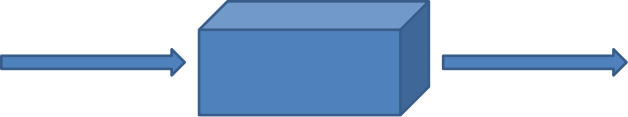
\includegraphics[width=.66\textwidth]{ch13/package.png}
        \end{figure}
    \end{itemize}
\end{frame}
%------------------------------------------------------------

\section{常用的函数}

%------------------------------------------------------------
\begin{frame}[fragile]
    \frametitle{常用的函数}

        \begin{tabular}{ccccc}
            \toprule
            函数名  & 功能 & 参数类型 & 返回值类型 & 头文件 \\
            \midrule
            \lstinline|sqrt(a)|  & 平方根 & 浮点数 & 浮点数 & \lstinline|cmath|  \\
            \lstinline|pow(a, n)| & 幂 & 浮点数 & 浮点数 & \lstinline|cmath|  \\
            \lstinline|abs(a)| & 绝对值 & 整数或浮点数 & 同参数类型 & \lstinline|algorithm|  \\
            \lstinline|max(a, b)| & 最大值 & 同类型参数 & 同参数类型 & \lstinline|algorithm|  \\
            \lstinline|min(a, b)| & 最小值 & 同类型参数 & 同参数类型 & \lstinline|algorithm|  \\
            \lstinline|swap(a, b)| & 交换变量 & 同类型参数 & 无 & \lstinline|utility|  \\
            \bottomrule
        \end{tabular}

        \begin{itemize}
            \item 示例
            \begin{itemize}
                \item<2-> 可用 \lstinline|sqrt(2)| 求 $\sqrt{2}$
                \item<3-> 可用 \lstinline|pow(2, 5)| 求 $2^5$
                \item<4-> 可用 \lstinline|abs(-2)| 求 $|-2|$
            \end{itemize}
        \end{itemize}
\end{frame}
%------------------------------------------------------------

\section{总结}

%------------------------------------------------------------
\begin{frame}[fragile]
    \frametitle{函数}

    \begin{itemize}
        \item<1-> 函数的定义
        
            \begin{itemize}
                \item 返回值类型、函数名、参数列表、函数体
            \end{itemize}

        \item<2-> 函数的调用
        
            \begin{itemize}
                \item 函数调用方式与跳转过程
                \item 形参、实参
                \item 多参数、有返回值函数调用注意要点
            \end{itemize}

        \item<3-> 常用的 C++ 库函数
    \end{itemize}
\end{frame}
%------------------------------------------------------------

%------------------------------------------------------------
\begin{frame}
    \begin{center}
        {\Huge Thank you!}
    \end{center}
\end{frame}
%------------------------------------------------------------

\end{document}
